% Prof. Dr. Ausberto S. Castro Vera
% UENF - CCT - LCMAT - Curso de Ci\^{e}ncia da Computa\c{c}\~{a}o
% Campos, RJ,  2024  
% Disciplina: An\'{a}lise e Projeto de Sistemas
% Aluno:

\chapterimage{ScalaH.jpg} % Table of contents heading image
\chapter{Projeto do Sistema}

Neste capítulo, apresentamos o projeto detalhado do sistema de estúdio de filmagem e edição, abordando desde as estratégias de implementação até a arquitetura completa do sistema. O projeto foi desenvolvido considerando as necessidades específicas de um estúdio moderno que utiliza tecnologias avançadas como câmera virtual, motion capture e scanning 3D.

\section{Estratégia do Projeto - Exemplos}

\subsection{Exemplo 1: Sistema Pronto - Autodesk ShotGrid}
Para o gerenciamento de produção e pipeline criativo, foi escolhido o Autodesk ShotGrid (anteriormente Shotgun), que oferece:
\begin{itemize}
    \item Sistema de rastreamento de produção integrado
    \item Gerenciamento de assets e versões
    \item Ferramentas de revisão e aprovação em tempo real
    \item Integração com principais softwares de edição e VFX
    \item Sistema de planejamento e cronograma de produção
\end{itemize}

\subsection{Exemplo 2: Sistema Terceirizado - AWS Media Services}
O sistema de computação em nuvem da Amazon Web Services foi selecionado para:
\begin{itemize}
    \item Renderização distribuída através do AWS Thinkbox Deadline
    \item Armazenamento escalável com Amazon S3 para arquivos brutos
    \item Streaming de mídia com AWS Elemental MediaConvert
    \item Sistema de backup redundante com AWS Glacier
    \item Processamento de machine learning para tracking automático
\end{itemize}

\subsection{Exemplo 3: Sistema Desenvolvido - Virtual Production Suite}
O sistema proprietário de produção virtual foi desenvolvido internamente para:
\begin{itemize}
    \item Integração com Unreal Engine para cenários virtuais em tempo real
    \item Sistema personalizado de controle de câmera virtual
    \item Pipeline de dados para motion capture com suporte Rokoko
    \item Interface de controle de LED wall sincronizada
    \item Sistema de preview em tempo real para diretores e produtores
\end{itemize}
       

\section{Refinamento dos Diagramas DFD e E-R}
%%%% Utilize os diagramas da Modelagem de procerssos para refinar

\section{Arquitetura do Sistema - Estilos}

\subsection{Arquitetura do Sistema}
A arquitetura geral do sistema segue um modelo distribuído com os seguintes componentes principais:
\begin{itemize}
    \item Central de Edição (12 estações com DaVinci Resolve Studio)
    \item Centro de Filmagem (LED Wall + Câmera Virtual Unreal Engine)
    \item Centro de Motion Capture (Rokoko SmartSuit Pro II + OptiTrack)
    \item Centro de Scanning (LIDAR + fotogrametria)
    \item Data Center (AWS + armazenamento local)
    \item Servidor Interno (gerenciamento via ShotGrid)
\end{itemize}

\begin{figure}[ht]
    \centering
    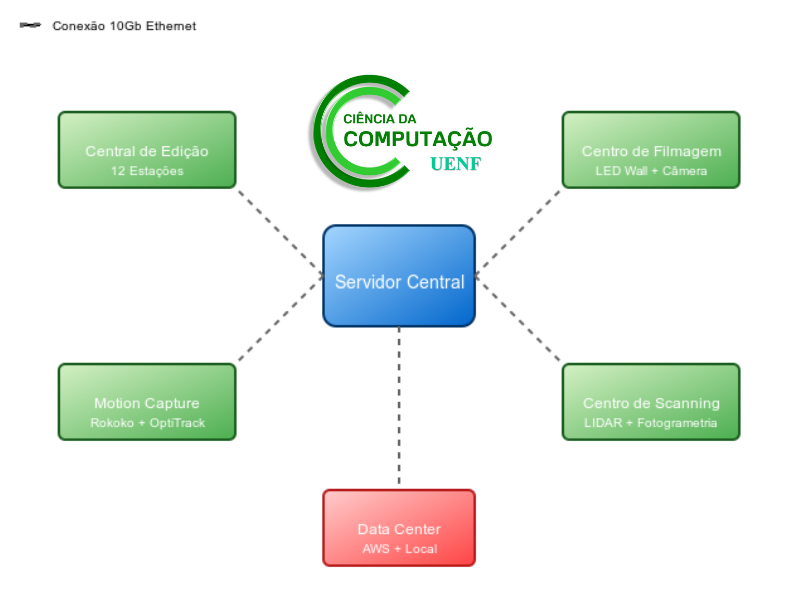
\includegraphics[width=0.8\textwidth]{Sistema}
    \caption{AAA}
    \label{fig:data}
\end{figure}

\subsection{Arquitetura do Hardware}
A infraestrutura de hardware é composta por:
\begin{itemize}
    \item Rede 10 Gigabit Ethernet Cisco para todas as estações
    \item Conexões de fibra ótica dedicadas ao servidor central
    \item Storage NetApp para armazenamento de alta performance
    \item Sistemas UPS redundantes APC
    \item Workstations Dell Precision com NVIDIA RTX
    \item LED Wall Samsung The Wall
\end{itemize}

\begin{figure}[ht]
    \centering
    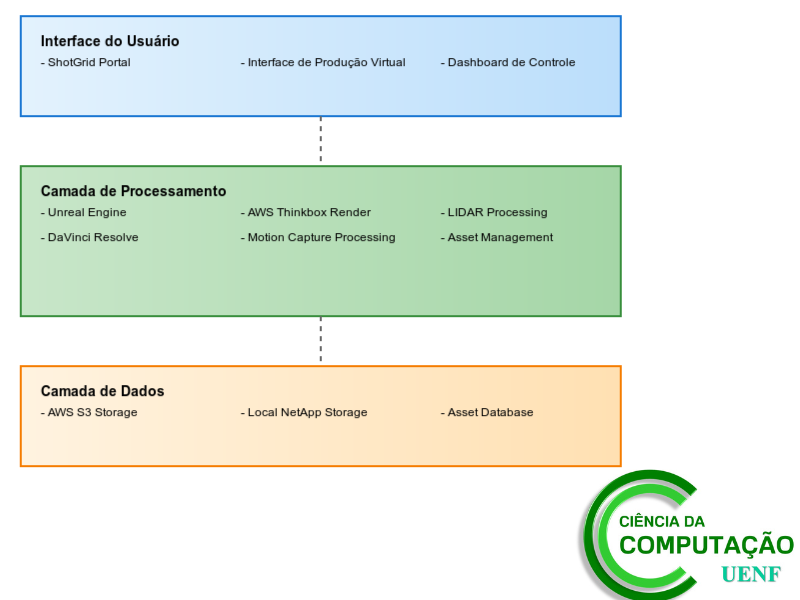
\includegraphics[width=0.8\textwidth]{Arquitetura}
    \caption{AAA}
    \label{fig:data}
\end{figure}

\pagebreak
\newpage

\subsection{Arquitetura de Software}
O sistema de software é estruturado em camadas:
\begin{itemize}
    \item Interface do usuário (ShotGrid + interface proprietária)
    \item Sistema de renderização (AWS Thinkbox + local)
    \item Unreal Engine para produção virtual
    \item DaVinci Resolve para pós-produção
    \item Sistema proprietário de controle de LED wall
    \item Pipeline de automação via Python e USD
\end{itemize}

\begin{figure}[ht]
    \centering
    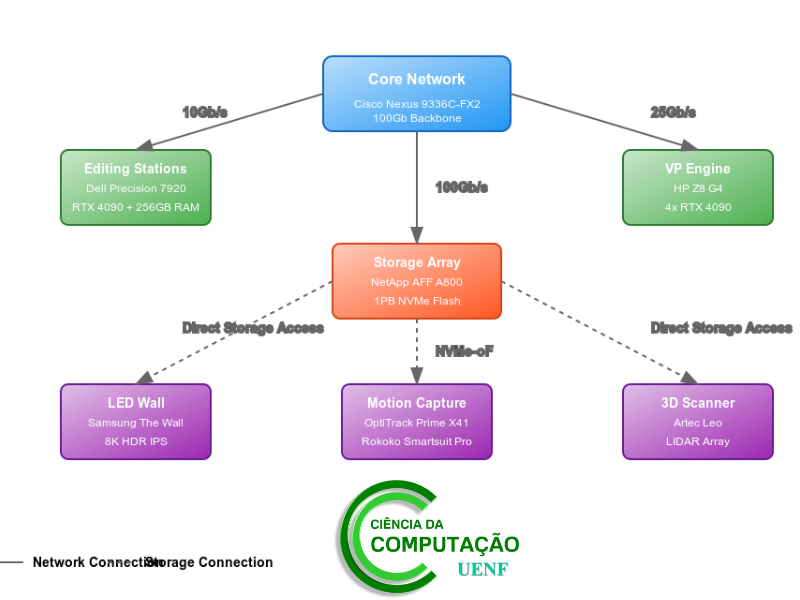
\includegraphics[width=0.8\textwidth]{Rede}
    \caption{AAA}
    \label{fig:data}
\end{figure}
